\begin{figure}[h] 
\centering 
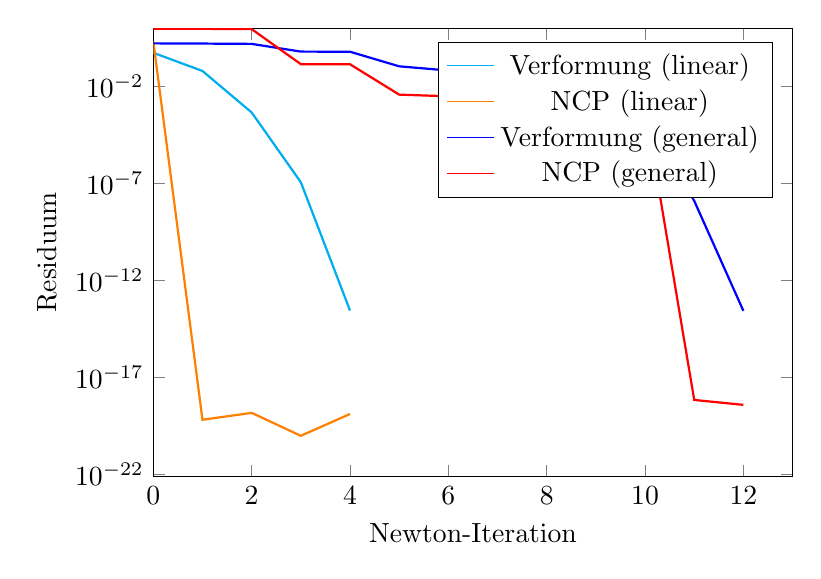
\begin{tikzpicture}[every plot/.append style={thick}] 
\begin{axis}[ 
label style={font=\normalsize}, 
xlabel={Newton-Iteration}, 
ylabel={Residuum}, 
xmin=0, xmax=13, 
ymode=log, 
ymin=0, ymax=10, 
width=0.8\textwidth, 
height=0.6\textwidth, 
legend pos=north east, 
legend style={cells={align=left}}, 
grid style=dashed, 
] 
\addplot[ 
color=cyan, 
] 
coordinates { 
(0, 5.42e-01)(1, 6.26e-02)(2, 4.57e-04)(3, 1.16e-07)(4, 2.85e-14)}; 
\addlegendentry{Verformung (linear)} 
\addplot[ 
color=orange, 
] 
coordinates { 
(0, 2.09e+00)(1, 6.71e-20)(2, 1.52e-19)(3, 1.00e-20)(4, 1.33e-19)}; 
\addlegendentry{NCP (linear)} 
\addplot[ 
color=blue, 
] 
coordinates { 
(0, 1.66e+00)(1, 1.62e+00)(2, 1.56e+00)(3, 6.25e-01)(4, 6.15e-01)(5, 1.09e-01)(6, 6.62e-02)(7, 6.48e-02)(8, 2.13e-02)(9, 3.53e-03)(10, 3.11e-04)(11, 1.27e-08)(12, 2.73e-14)}; 
\addlegendentry{Verformung (general)} 
\addplot[ 
color=red, 
] 
coordinates { 
(0, 9.44e+00)(1, 9.30e+00)(2, 9.00e+00)(3, 1.41e-01)(4, 1.39e-01)(5, 3.79e-03)(6, 3.11e-03)(7, 3.06e-03)(8, 3.10e-03)(9, 3.10e-03)(10, 8.63e-04)(11, 7.03e-19)(12, 3.93e-19)}; 
\addlegendentry{NCP (general)} 
\end{axis} 
\end{tikzpicture} 
\caption{Residuen des Stoffgesetzes 'Neo Hooke' mit Hinderniss 'Hut' und 8450 Freiheitsgraden für die Verschiebung.} 
\label{fiq:NeoHooke_Hut_level5} 
\end{figure} 
